\documentclass[tikz]{standalone}
\usetikzlibrary{arrows, positioning}
\tikzset{
  treenode/.style = {align=center, inner sep=1pt, text centered,
    font=\sffamily},
  bst/.style = {treenode, circle, black, font=\sffamily\bfseries, draw=black, text width=2em}
}
\begin{document}
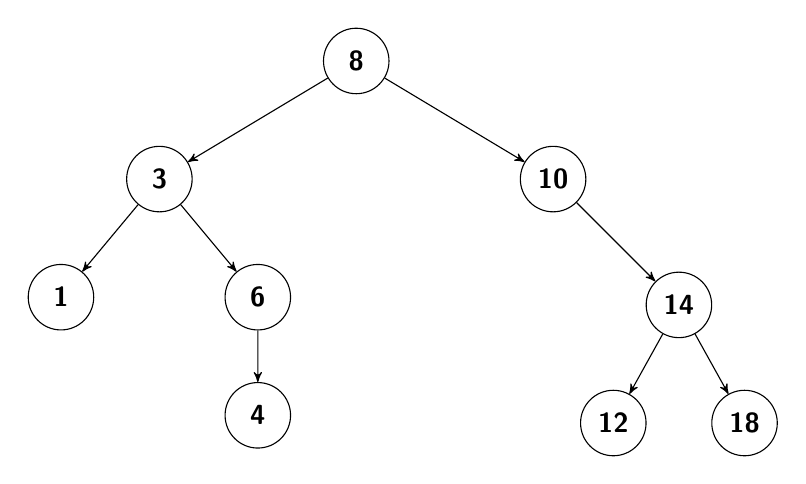
\begin{tikzpicture}[->,>=stealth',level/.style={sibling distance = 5cm/#1,
  level distance = 1.5cm}]
\node [bst] {8}
    child {node [bst] {3}
        child {node [bst] {1}}
        child {node [bst] {6}
            child {node [bst] {4}}
        }
    }
    child {node (n10) [bst] {10}
        child {node [bst, below right=of n10] {14}
            child {node [bst] {12}}
            child {node [bst] {18}}
        }
    }
;
\end{tikzpicture}
\end{document}
